\documentclass[border=0.125cm]{standalone}
\usepackage{tikz}
\usepackage{pgfplots}
\usepackage{graphicx}

\usetikzlibrary{decorations.pathmorphing}
\pgfplotsset{compat=newest}
\usetikzlibrary{shapes.geometric,arrows,fit,matrix,positioning}
\tikzset{main node/.style={circle,fill=black!20,draw,minimum size=3.5mm,inner sep=0pt},
         every node/.style={circle,fill=black,draw,minimum size=1mm,inner sep=0pt,label distance=-1mm},
         subtree/.style={isosceles triangle,fill=blue!20,draw,minimum size=4mm,inner sep=0pt,shape border rotate=90},
         edge label/.style = {rectangle,draw=none,fill=none}
}
\begin{document}
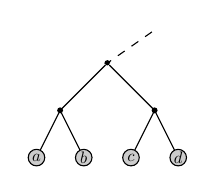
\begin{tikzpicture}[-,>=stealth', 
level 1/.style={sibling distance = 20mm},
level distance = 0.7cm, 
scale=0.6,
transform shape]
\node[edge label] {}
child[dashed]{
    [level distance = 1cm]node (0) {}
        child[solid]{
            [sibling distance = 10mm] node (1) {}
                child{
                    node [main node] (2) {$a$}
                }
                child{
                    node [main node] (3) {$b$}
                }
        }
        child[solid]{
            [sibling distance = 10mm] node (1) {}
                child{
                    node [main node] (4) {$c$}
                }
                child{
                    node [main node] (5) {$d$}
                }
        }
}
child[missing]{node {}}
;
\end{tikzpicture}

\end{document}






